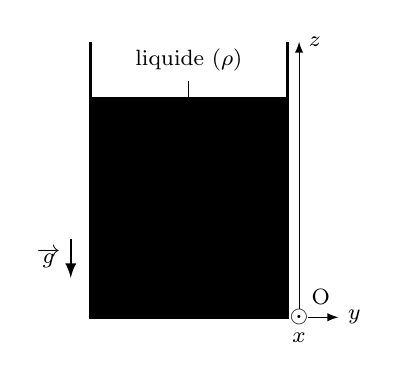
\begin{tikzpicture} [
	scale=0.5,
	font=\footnotesize,
    vecteur/.style={-latex,thick},
    liquide/.style={fill=\JRLblueC,very thin,draw=\JRLblueF},
	]
%	\shadedraw[color=gray,top color=white,bottom color=gray] (-2.5,5.6)--++(0,-5.6)--++(5,0)--++(0,5.6)--cycle;
	\draw[liquide] (-2.5,5.6)--++(0,-5.6)--++(5,0)--++(0,5.6)--cycle;
	\draw[line width=1pt] (-2.5,7)--++(0,-7)--++(5,0)--++(0,7);
	\draw[-] (0,5)--++(0,1) node[above]{liquide ($\rho$)};
	\draw[vecteur] (-3,2)--++(0,-1) node[pos=0.5,left]{$\overrightarrow{g}$};
	\draw[|<->|,shift={(-1,0)}](0,5.6)--++(0,-5.6) node[midway, left]{$h_{0}$};
	\draw (-.3,2)node{•}node[right]{M$(x,y,z)$};
	\draw[->,>=latex,shift={(2.8,0)}](0,0)node[above right=1pt]{O}--++(0,7)node[right]{$z$};
	\draw[->,>=latex,shift={(2.8,0)}](0,0)--++(1,0)node[right]{$y$};
	\draw[shift={(2.8,0)}](0,0)node[fill=white,inner sep=0]{$\odot$}node[below=2pt]{$x$};
\end{tikzpicture}